\documentclass[a4paper]{article}

%opening

\title{\huge Assignment 1: Software Requirements Specification and Technology Neutral Process Design
	\\COS 301 Team Alpha Project
	\\Version 1.0}

\author{\\\\Amy Lochner 14038600\\ Avinash Singh 14043778 \\
	Christiaan Nel 14029368\\ Christiaan Saaiman 12059138 \\
	Gerard van Wyk 14101263\\ Marc Antel 12026973\\
	Themba Mbhele 14007950
	\\
	\\
	\\\textit{https://github.com/AvinashSingh786/COS301-Alpha.git}
	\\
	\\
	\\ University Of Pretoria\\}

\date{February 2016}

\usepackage{graphicx}
\usepackage{float}

\begin{document}
	
	\maketitle

	\pagenumbering{gobble}
	\newpage

	\tableofcontents
	\pagenumbering{arabic}
	\newpage
	
	\section{Introduction}
	
	This document defines the Software Requirements Specification and Technology Neutral Process Design for COS 301 Team Alpha. The Computer Science Department has expressed a need for the creation of a system, which can allow researchers to keep track of publications which they are currently working on, or have already published.
	\\
	The aim of this project is to follow a structured software development process in order to produce a product which provides the client with all the required functionality in an elegantly designed and built product. A collaborative and co-operative approach is required between all stakeholders who are involved in this project. 
	\\
	The information, specifications, and diagrams within this document are presented in order to provide testable requirements which correlate to the client's needs.
	
	\section{Vision}
	The client for this project, Ms. Vreda Pieterse who is a member of the Department of Computer Science at the University of Pretoria, has solicited us to develop a system. The purpose of this system is to record and oversee all publications of staff members or research groups, within the Department of Computer Science. The system will assist the Head of Department to track the progress on any papers which are in the process of being written; as well as determining whether or not a staff member is under performing thus allowing the Head of Department the opportunity to provide advice to these staff members.
	
	\section{Background}
	\subsection{The client's problem}
	The client has solicited us to develop a system that has specific usability goals, as well as certain user-experience goals. Currently, the Department of Computer Science does not have a system with which to monitor the progress of staff member's publications, nor to keep track of how many publications an author is working on. Furthermore, it is necessary to determine which publications will be presented at different conferences, as well as the reporting capabilities, and the ability to remind users of deadlines. The system should provide all these requirements in a secure, flexible and intuitive manner.
	
	\subsection{Future business/research opportunities}
	It is desired that this system will encourage authors to collaborate with other authors on similar topics and to expand the users base knowledge of ongoing research projects.
	\\
	\\
	\\
	
	
	\section{Architecture Requirements}
	This section will be expanded on and developed further in the next phase of the project design and will be mentioned only briefly here.
	\\
	\subsection{Access Channel Requirements}
	As it is possible that the system may have concurrent users, it is favourable that there be interfaces such as a web application or website, as well as a mobile platform applications for the various different mobile devices through which the system can be accessed.
	\\
	\subsection{Quality Requirements}
	Specify and quantify each of the quality requirements which are relevant to the system
	\begin{itemize}
		\item Performance - How well the system can cope with extreme load.
		\item Security - Minimising the possibility of leaking information, maintaining data integrity, and avoiding session hijacking.
		\item Maintainability - Can the system be managed without downtime.
		\item Scalability - Can the system be used for large amount of users without it affecting performance.
		\item Efficiency - Can the system be optimized to produce faster and better results.
		\item Flexibility - Can the system be easily changed or modified.
		\item Reliability - Is the system able to cope with the load in order to  provide constant access, ensure the system is always active and can provide all functionality.
		\item Integrability - Will the system be able to integrate with other technologies.
		\item User Friendly - Does a user easily understand how to use the system.
		\item Concurrency - Can multiple users perform actions at the same time.
		\item Low Cost, Reduced data usage - Is it suitable for users with low budget and capped Internet.
		\item Updatability - Can the system have version updates to introduce new features or functionality whilst maintaining old data.
		\\
	\end{itemize}
	
	\subsection{Integration Requirements}
	This section specifies any integration requirements for any external systems. This may include
	\begin{itemize}
		\item The different Web protocols used.
		\item API - UML Interfaces.
		\item Google Calender and Email integration.
		\item Mobile Scalability and functionality Integration.
		\item Venue and Publication integration.
		\\
	\end{itemize}
	
	\subsection{Architecture Constraints}
	This specifies any constraints, the client may require, to be placed on the system architecture. Such constraints may be:
	\begin{itemize}
		\item HTML (Hypertext Markup Language)
		\item AJAX (Asynchronous JavaScript and XML)
		\item JavaEE (Java Platform Enterprise Edition)
		\item JavaScript (Functionality to HTML)
		\item PHP (Server Side Scripting)
		\item MySQL (Database Manager)
		\item Android (Mobile Devices)
		\item IOS (Mobile Devices)
		\item Apache (Web Server)
		\item Linux/Windows (Operating System)
		\\
		\\
	\end{itemize}
	\pagebreak
	\section{Functional Requirements and Application Design}
	This section discusses the application functionality required by users.
	\subsection{Use Case Prioritization}
	\subsubsection{User Login}
	\textbf{Description:}  A user is required to log into the system before the user can make use of any functionality.
	\\
    \textbf{Prioritisation:} Critical\\
    
    
      \textbf{Pre-conditions}
    \begin{itemize}
        \item A user must have a connection to the server.
        \item A user must be registered as a user by a person with HOD or Admin permission.
        \item The user must enter the correct information in order for the authentication to be successful.
    \end{itemize}
    
    \textbf{Post-conditions}
     \begin{itemize}
        \item The user has specific access to the server on which all data is stored, i.e add/edit authors and search for authors
        \item The user is able to use all the user functionality provided by the system 
        \item The user may log out of the system when they wish to.
    \end{itemize}
    
    \pagebreak
    
    \subsubsection{User Registration}
    
    \textbf{Description:}  In order to be able to log into the system and make use of the functionality provided by the system the user must be registered on the system. \\
    \textbf{Prioritisation:} Critical\\
   
    \textbf{Pre-conditions}
     \begin{itemize}
        \item The user must be part of the staff of the Computer Science Department of the University of Pretoria.
        \item The administrator or HOD of the system must have registered the user on the system.
        \item The user must decide on their login credentials.
   \end{itemize}
    
    \textbf{Post-conditions}
    \begin{itemize}
        \item The user's login information is securely stored in the system database.
        \item The user can log into the system.
    \end{itemize}
    
    	\begin{figure}[H]
    		\centering
    		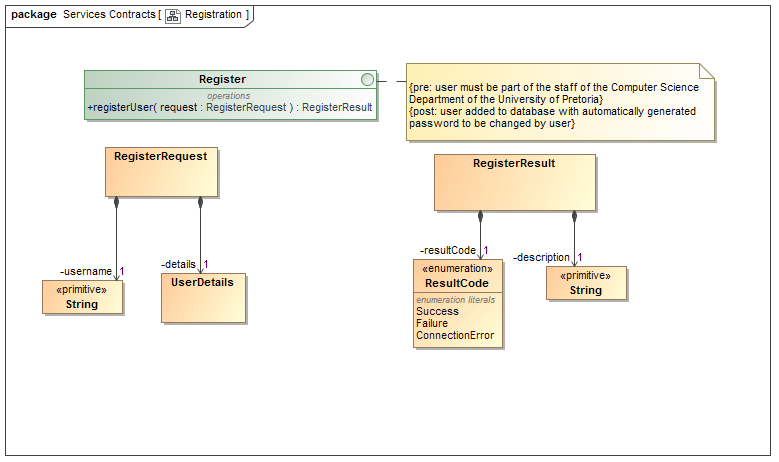
\includegraphics[width=\textwidth]{5.1.2.Registration.Services.Contract.png}
    		\caption{Service Contract: User Registration}
    	\end{figure}
    
    
    \pagebreak
    \subsubsection{Update User}
   
    \textbf{Description:} Personal details as well as log in credentials can be changed if and when necessary.\\
     \textbf{Prioritisation:} Important\\
     
    \textbf{Pre-conditions}
     \begin{itemize}
        \item The administrator or HOD must be logged into the system.
        \item The user to be updated must already exist in the system.
        \item The administrator or HOD must have the new information.
   \end{itemize}
    
    \textbf{Post-conditions}
    \begin{itemize}
        \item The user's information is updated on the system's database.
    \end{itemize}
    
        	\begin{figure}[H]
        		\centering
        		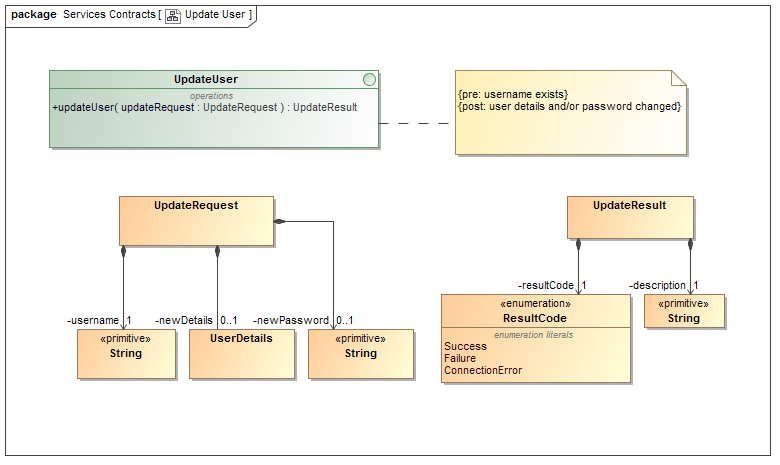
\includegraphics[width=\textwidth]{5.1.3.Update.User.Services.Contract.png}
        		\caption{Service Contract: Update User}
        	\end{figure}
    \pagebreak
    \subsubsection{Remove User}
    
    \textbf{Description:} Should a user no longer belong to the Department of Computer Science the person should be removed from the system.\\
    \textbf{Prioritisation:} Important\\
    
    \textbf{Pre-conditions}
     \begin{itemize}
        \item The person should be a user on the system.
        \item The person should no longer belong to the staff of the Department of Computer Science.
        \item The administrator or HOD must be the logged in.
   \end{itemize}
    
    \textbf{Post-conditions}
    \begin{itemize}
        \item The person is removed from the system's database.
        \item The person can no longer gain access to the system.
        \item The person history still remains in the log file.
    \end{itemize}

    	\begin{figure}[H]
    		\centering
    		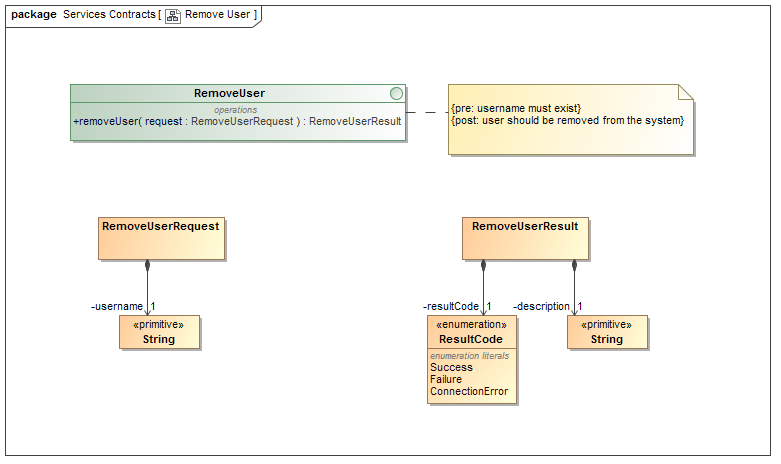
\includegraphics[width=\textwidth]{5.1.4.Remove.User.Services.Contract.png}
    		\caption{Service Contract: Remove User}
    	\end{figure}
\pagebreak
    \subsubsection{Create Publication}
    
    \textbf{Description:} Adding a paper to the system\\
    \textbf{Prioritisation:} Critical\\
    
    
    \textbf{Pre-conditions}
     \begin{itemize}
        \item The user(may be the administrator or HOD) should be logged into the system.
        \item The user, if not the administrator or HOD, must be a contributor to the paper.
        \item All authors who contributed to the paper should be available on the system.
   \end{itemize}
    
    \textbf{Post-conditions}
    \begin{itemize}
        \item The paper is added to the system
    \end{itemize}
    
        	\begin{figure}[H]
        		\centering
        		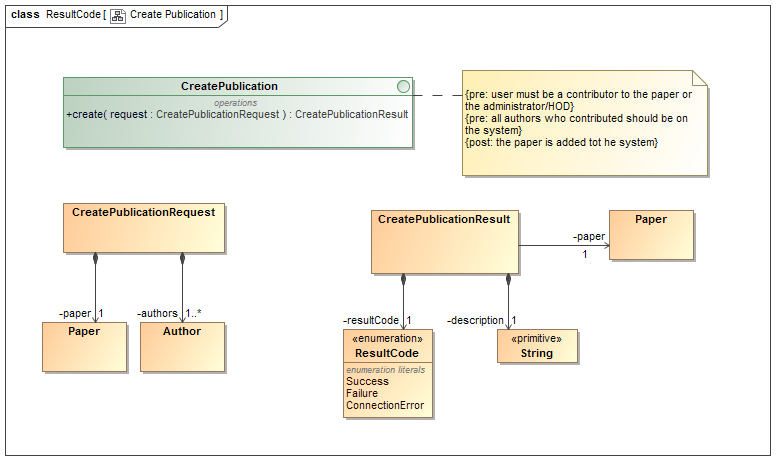
\includegraphics[width=\textwidth]{5.1.5.Create.Publication.Services.Contract.png}
        		\caption{Service Contract: Create Publication}
        	\end{figure}
\pagebreak
    \subsubsection{Update Publication}
    
    \textbf{Description:} Allows a user/administrator/HOD to change a publication's meta-data\\
    \textbf{Prioritisation:} Critical\\
    \\
    
    \textbf{Pre-conditions}
     \begin{itemize}
        \item The user(may be the administrator or HOD) should be logged into the system.
        \item The user, if not the administrator or HOD, must be a contributor to the paper.
        \item The paper must already be in the system.
   \end{itemize}
    
    \textbf{Post-conditions}
    \begin{itemize}
        \item The paper's meta-data is updated
    \end{itemize}
    
        	\begin{figure}[H]
        		\centering
        		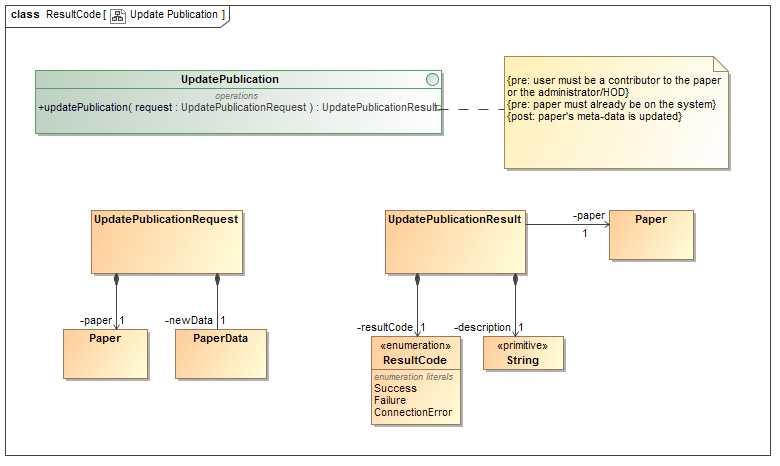
\includegraphics[width=\textwidth]{5.1.6.Update.Publication.Services.Contract.png}
        		\caption{Service Contract: Update Publication}
        	\end{figure}
    \pagebreak
    \subsubsection{View Publication}
    
    \textbf{Description:} Allows a user/administrator/HOD to view the meta-data of a paper that lies within their permissions\\
    \textbf{Prioritisation:} Important\\
    \\
    
    \textbf{Pre-conditions}
     \begin{itemize}
        \item The user(may be the administrator or HOD) should be logged into the system.
        \item The user - if not the administrator, HOD or research leader - must be a contributor to the paper.
        \item The paper must already be in the system.
   \end{itemize}
    
    \textbf{Post-conditions}
    \begin{itemize}
        \item The paper's meta-data is displayed to the user
    \end{itemize}
    
            	\begin{figure}[H]
            		\centering
            		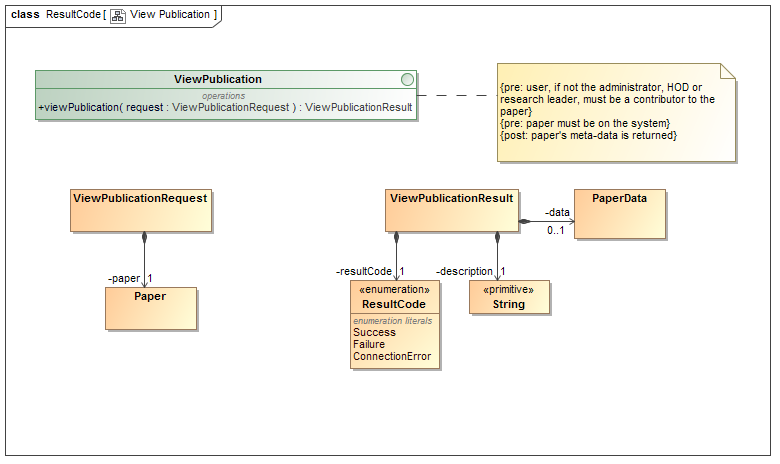
\includegraphics[width=\textwidth]{5.1.7.View.Publication.Services.Contract.png}
            		\caption{Service Contract: View Publication}
            	\end{figure}
    
\pagebreak

    \subsubsection{Add Publication Type}

    \textbf{Description:} Allows the administrator or HOD to add a publication type \\
        \textbf{Prioritisation:} Important\\
        \\
        
        
    \textbf{Pre-conditions}
     \begin{itemize}
        \item The user(must be the administrator or HOD) should be logged into the system.
        \item The publication type to add must not already be in the system.
   \end{itemize}
    
    \textbf{Post-conditions}
    \begin{itemize}
        \item The new publication type is added to the system.
    \end{itemize}
    
        
        \begin{figure}[H]
        	\centering
        	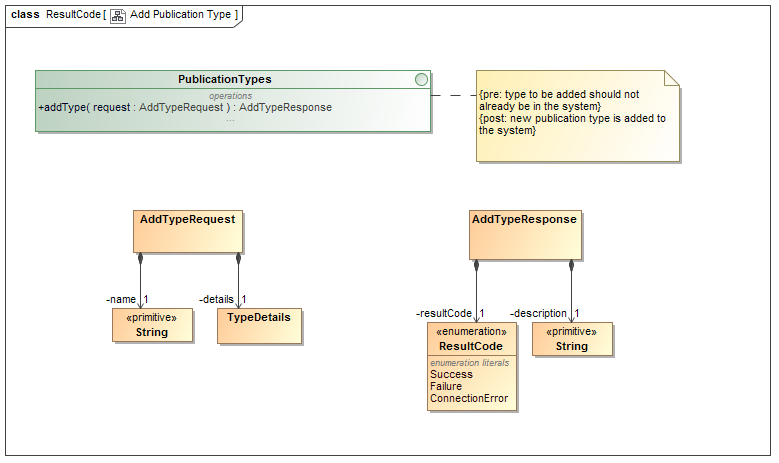
\includegraphics[width=\textwidth]{5.1.8.Add.Publication.Type.Services.Contract.png}
        	\caption{Service Contract: Add Publication}
        \end{figure}
    
    \pagebreak
    \subsubsection{Update Publication Type}
    
    \textbf{Description:} Allows the administrator or HOD to update a publication type's details\\
    \textbf{Prioritisation:} Important\\
    
    
    \textbf{Pre-conditions}
     \begin{itemize}
        \item The user(must be the administrator or HOD) should be logged into the system.
        \item The user - if not the administrator, HOD or research leader - must be a contributor to the paper.
        \item The publication type to be updated must already be in the system.
   \end{itemize}
    
    \textbf{Post-conditions}
    \begin{itemize}
        \item The selected publication type will be updated with the new information.
    \end{itemize}
    
            \begin{figure}[H]
            	\centering
            	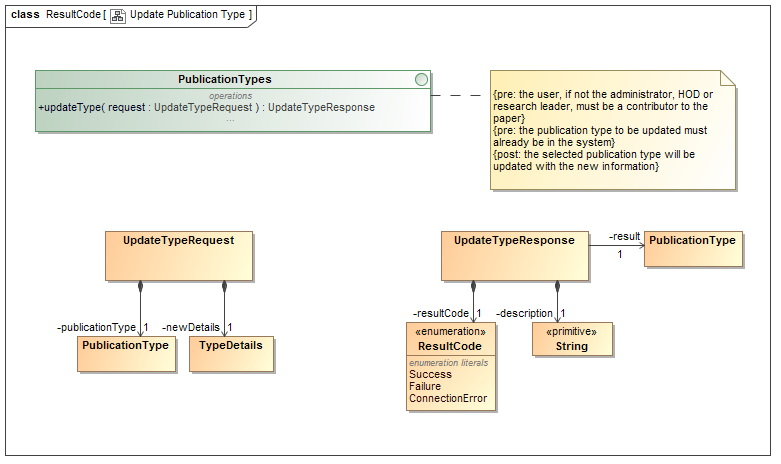
\includegraphics[width=\textwidth]{5.1.9.Update.Publication.Type.Services.Contract.png}
            	\caption{Service Contract: Update Publication}
            \end{figure}
    
    \pagebreak
    \subsubsection{Add Reminder}
        \textbf{Description:} Allows the user to create a reminder for the deadline of the publication.\\
        \textbf{Prioritisation:} Nice-To-Have.
        \\
        
        \textbf{Pre-conditions}
        \begin{itemize}
        	\item The user(can be the HOD) should be logged into the system.
        	\item The user must be a contributor to the paper.
        	\item The publication must already be in the system.
        \end{itemize}
        
        \textbf{Post-conditions}
        \begin{itemize}
        	\item A reminder via Mail or Calendar will be set with the selected publication and deadline.
        \end{itemize}
    \pagebreak
	\subsubsection{Create Research Group}
	\textbf{Description:} Allows the administrator or HOD to create a new Research Group\\
	\textbf{Prioritisation:} Critical\\
	
	\textbf{Pre-conditions}
	 \begin{itemize}
		\item The user(must be the administrator or HOD) should be logged into the system.
		\item The Research Group you wish to create must not already be in the system.
	\end{itemize}
	
	\textbf{Post-conditions}
	 \begin{itemize}
		\item The Research Group will be created and stored in the database.
		\item Users will be able to join the Research Group.
		\item Research Leader will be able to see all Publications made by the Research Group's members.
	\end{itemize}
	\pagebreak
	\subsubsection{View Research Group}
	\textbf{Description:} View the details of a Research Group \\
	\textbf{Prioritisation:} Nice-To-Have\\
	
	\textbf{Pre-conditions}
	 \begin{itemize}
		\item The user(must be the administrator or HOD) should be logged into the system.
		\item The Research Group must already exist in the database.
    \end{itemize}
	
	\textbf{Post-conditions}
	 \begin{itemize}
		\item The user will be able to view the details of the Research Group.
	\end{itemize}
	\pagebreak
	\subsubsection{Update Research Group}
	\textbf{Description:} Allows the administrator or HOD to update an existing Research Group\\
	\textbf{Prioritisation:} Important\\
	
	\textbf{Pre-conditions}
	 \begin{itemize}
		\item The user(must be the administrator or HOD) should be logged into the system.
		\item The Research Group must already exist in the database.
	\end{itemize}
	
	\textbf{Post-conditions}
	 \begin{itemize}
		\item The user will be able to edit and save the new information entered.
	\end{itemize}
	\pagebreak
	\subsubsection{Remove Research Group}
	\textbf{Description:} Allows the administrator or HOD to remove an existing Research Group\\
	\textbf{Prioritisation:} Important\\
	
	\textbf{Pre-conditions}
	 \begin{itemize}
		\item The user(must be the administrator or HOD) should be logged into the system.
		\item The Research Group must already exist in the database.
		\item The Research Group must have no members in it and no Research Leader.
	\end{itemize}
	
	\textbf{Post-conditions}
	 \begin{itemize}
		\item The user will be able to remove the Research Group from the database.
	\end{itemize}
	\pagebreak
	\subsubsection{Create Author}
	\textbf{Description:} Allows the user to create a new Author\\
	\textbf{Prioritisation:} Critical\\
	
	\textbf{Pre-conditions}
	 \begin{itemize}
		\item The user should be logged into the system.
		\item The Author must not already exist in the database.
	\end{itemize}
	
	\textbf{Post-conditions}
	 \begin{itemize}
		\item The user will be able to create a new Author and save him/her in the database.
	\end{itemize}
	\pagebreak
	\subsubsection{Update Author}
	\textbf{Description:} Allows the user to update an existing Author\\
	\textbf{Prioritisation:} Important\\
	
	\textbf{Pre-conditions}
	 \begin{itemize}
		\item The user should be logged into the system.
		\item The Author must already exist in the database.
	\end{itemize}
	
	\textbf{Post-conditions}
	 \begin{itemize}
		\item The user will be able to edit and save the new information entered.
	\end{itemize}
    \pagebreak
    \subsubsection{Generate Report}
	\textbf{Description:} Allows the user generate a report based on certain data\\
	\textbf{Prioritisation:} Nice to have\\
	
	\textbf{Pre-conditions}
	 \begin{itemize}
		\item The user should be logged into the system.
		\item There should be existing data in the system's database
 	\end{itemize}
	
	\textbf{Post-conditions}
	 \begin{itemize}
		\item The system will generate a report based on certain criteria and make it visible to the user
	\end{itemize}
	
    \pagebreak
	\subsection{Use Case/Services Contracts}
	
	\subsection{Required Functionality}
	\subsubsection{User-Research System interaction}
	\paragraph{\textbf{Description:} The type of user indicates what privileges that user has in the Research system}
	\paragraph{\textbf{Normal-user}}
	\begin{description}
		\item[$\bullet$] A normal user may log in to the system if registered on the system.
		\item[$\bullet$] A normal user may add publications to the system.
		\item[$\bullet$] A normal user must be an author of a publication should they want to add it to the system.
		\item[$\bullet$] A normal user may add authors to a publication.
		\item[$\bullet$] A normal user may change authors in a publication.
		\item[$\bullet$] A normal user may add a publication to a conference.
		\item[$\bullet$] A normal user may only view their own publications.
	\end{description}
	\paragraph{\textbf{Head of Department}}
	\begin{description}
		\item[$\bullet$] The head of department may log in to the system.
		\item[$\bullet$] The head of department may add/edit/remove a user.
		\item[$\bullet$] The head of department may add/edit/remove an author.
		\item[$\bullet$] The head of department may add publication/edit a publication.
		\item[$\bullet$] The head of department may be an author on a publication.
		\item[$\bullet$] The head of department may add authors to a publication.
		\item[$\bullet$] The head of department may add/remove publications for conferences.
		\item[$\bullet$] The head of department may view all publications on the system.
	\end{description}
	\paragraph{\textbf{Admin}}
	\begin{description}
		\item[$\bullet$] Admin users may log in to the system.
		\item[$\bullet$] Admin users may add/remove/edit users.
		\item[$\bullet$] Admin users may add/edit publications.
		\item[$\bullet$] Admin users may not be an author to any publication on the system.
		\item[$\bullet$] Admin users may add authors to a publication.
		\item[$\bullet$] Admin users may change authors to a publication.
		\item[$\bullet$] Admin users may add/remove publications to conferences.
		\item[$\bullet$] Admin users may view all publications on the system.
	\end{description}
	\begin{figure}[H]
		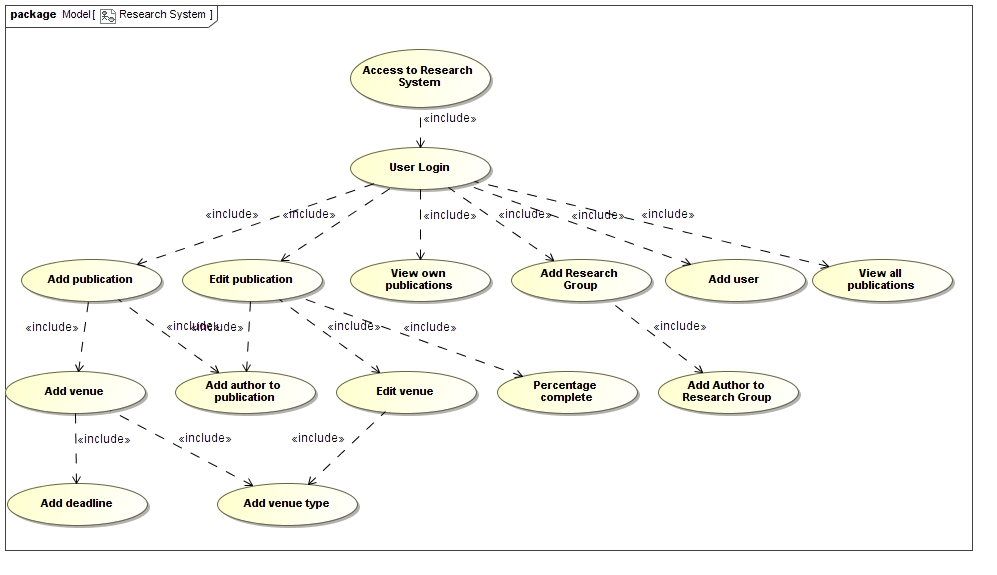
\includegraphics[width=\textwidth]{Overview.jpg}
		\caption{Functional Requirements: Overview of Research System \label{overflow}}
	\end{figure}
	\begin{figure}[H]
		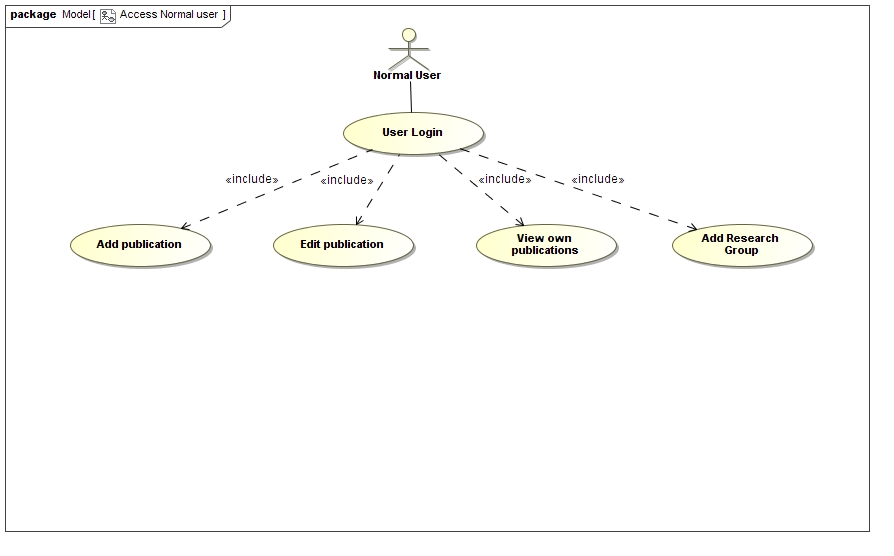
\includegraphics[width=\textwidth]{AccessNormaluser.jpg}
		\caption{Functional Requirements: Normal user access privileges \label{overflow}}
	\end{figure}
	\begin{figure}[H]
		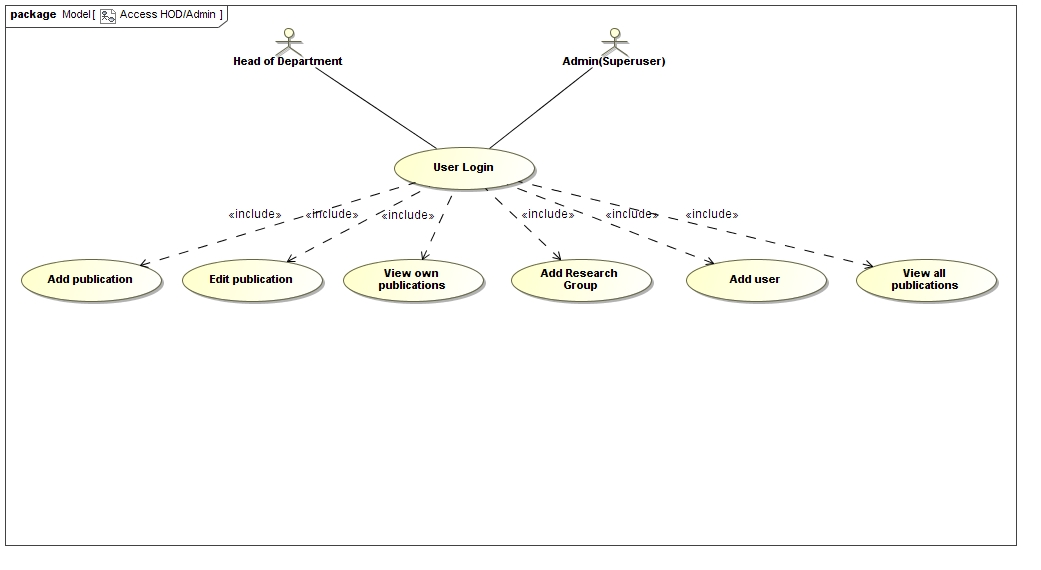
\includegraphics[width=\textwidth]{AccessHODAdmin.jpg}
		\caption{Functional Requirements: Superuser(HOD and admin) access privileges \label{overflow}}
	\end{figure}
		\subsection{Process Specification}
	This section conatins UML activity diagrams that illustrate the sequences that will be followed for various use case scenarios.
	\begin{figure}[H]
	    \centering
	    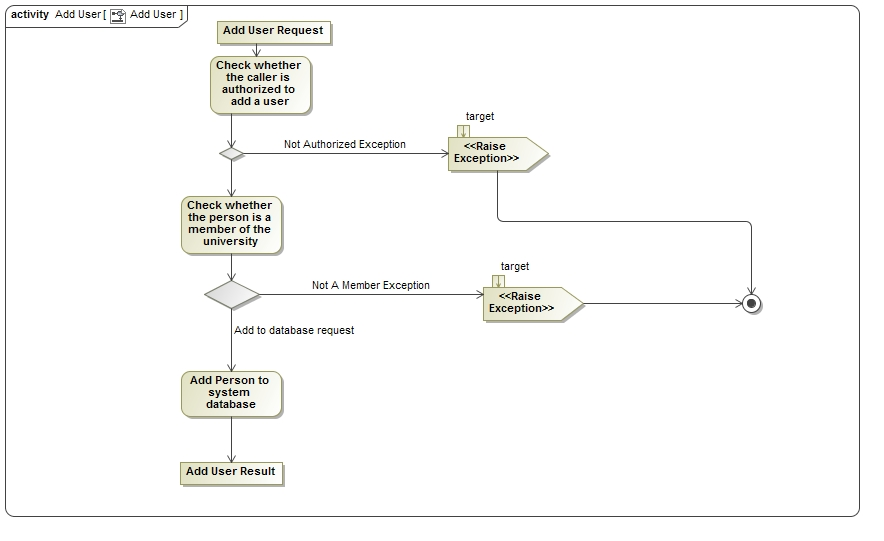
\includegraphics[width=\textwidth]{AddUser.jpg}
	    \caption{Process Specification: Adding A User}
	\end{figure}
	\begin{figure}[H]
	    \centering
	    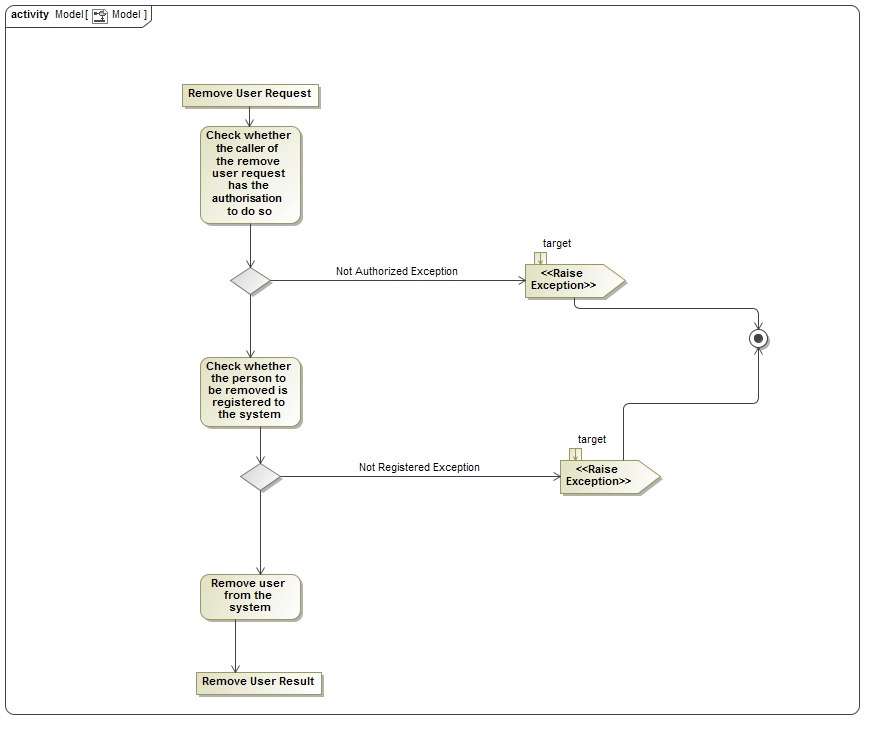
\includegraphics[width=\textwidth]{removeUser.jpg}
	    \caption{Process Specification: Removing A User}
	\end{figure}
	\begin{figure}[H]
	    \centering
	    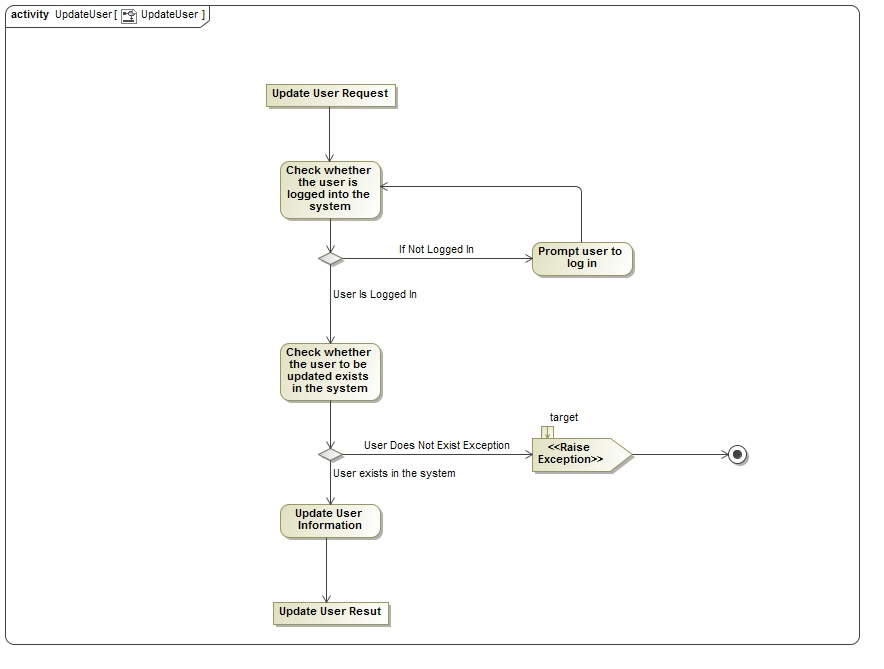
\includegraphics[width=\textwidth]{UpdateUser.jpg}
	    \caption{Process Specification: Update A User}
	\end{figure}
		\begin{figure}[H]
	    \centering
	    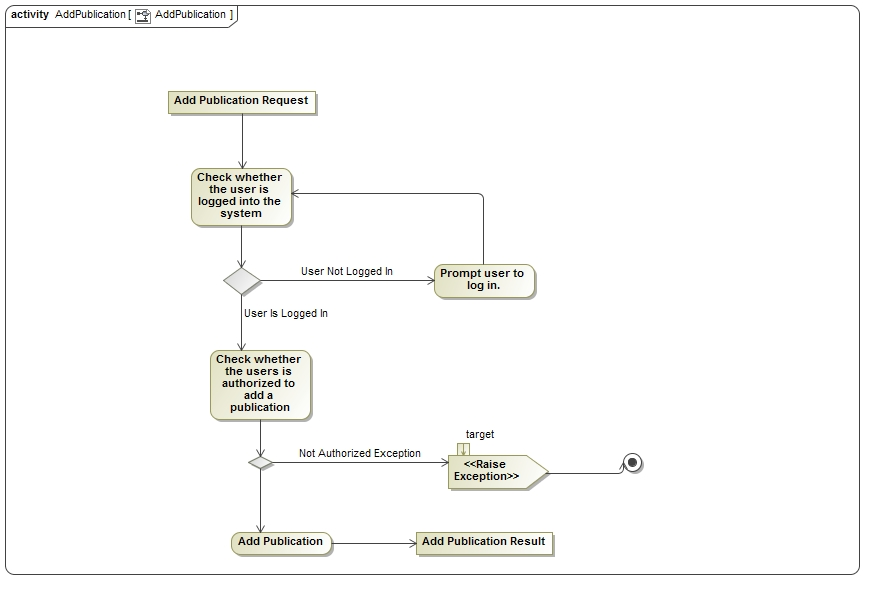
\includegraphics[width=\textwidth]{AddPublication.jpg}
	    \caption{Process Specification: Adding A Publication}
	\end{figure}
		\begin{figure}[H]
	    \centering
	    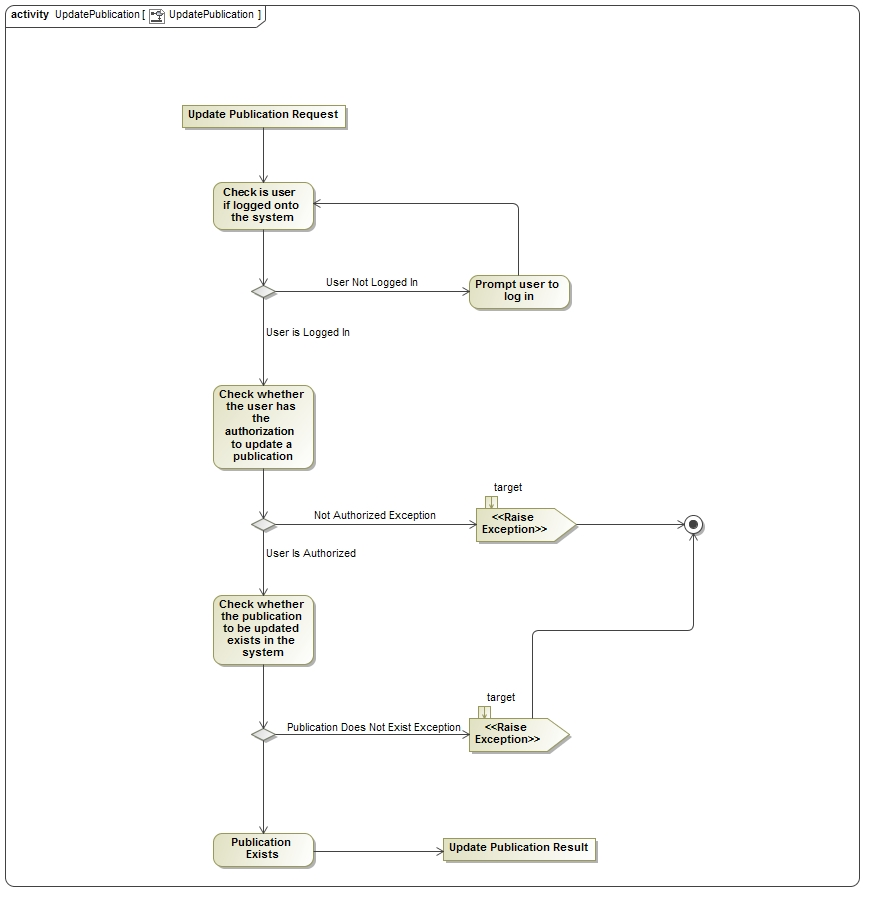
\includegraphics[width=\textwidth]{UpdatePublication.jpg}
	    \caption{Process Specification: Update A Publication}
	\end{figure}
		\begin{figure}[H]
	    \centering
	    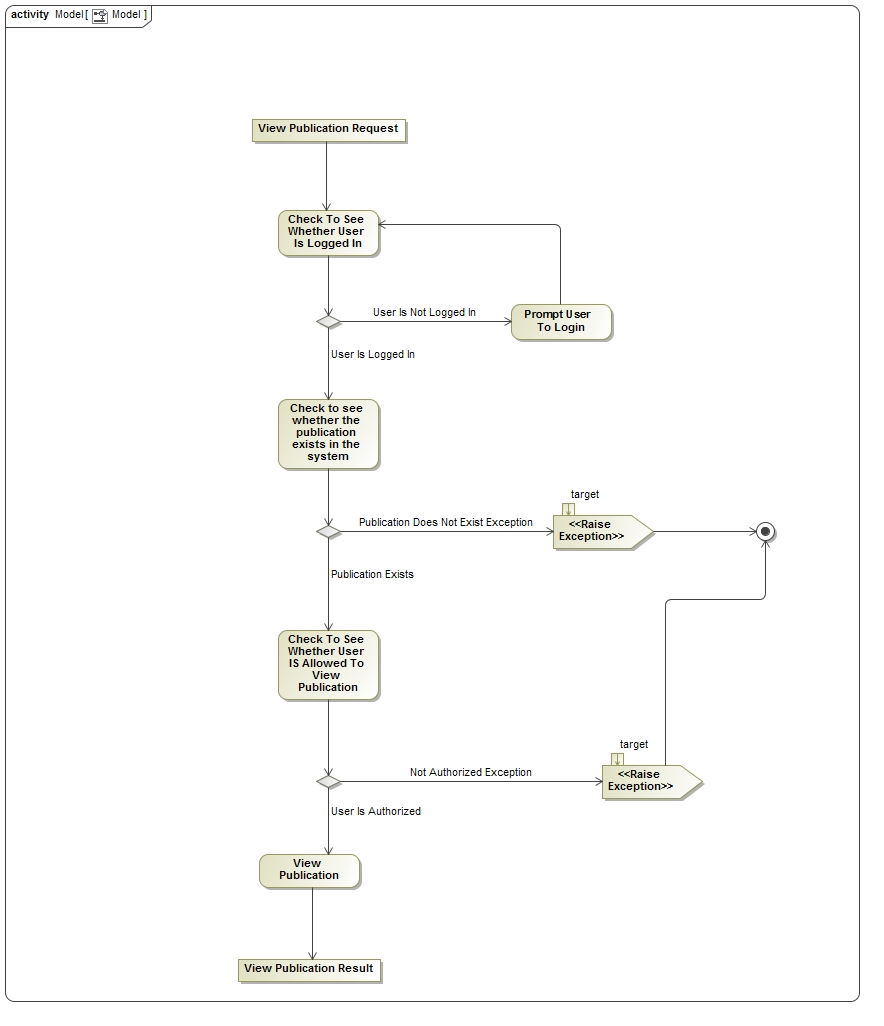
\includegraphics[width=\textwidth]{ViewPublication.jpg}
	    \caption{Process Specification: View A Publication}
	\end{figure}
	\subsection{Domain Model}
	\begin{figure}[H]
		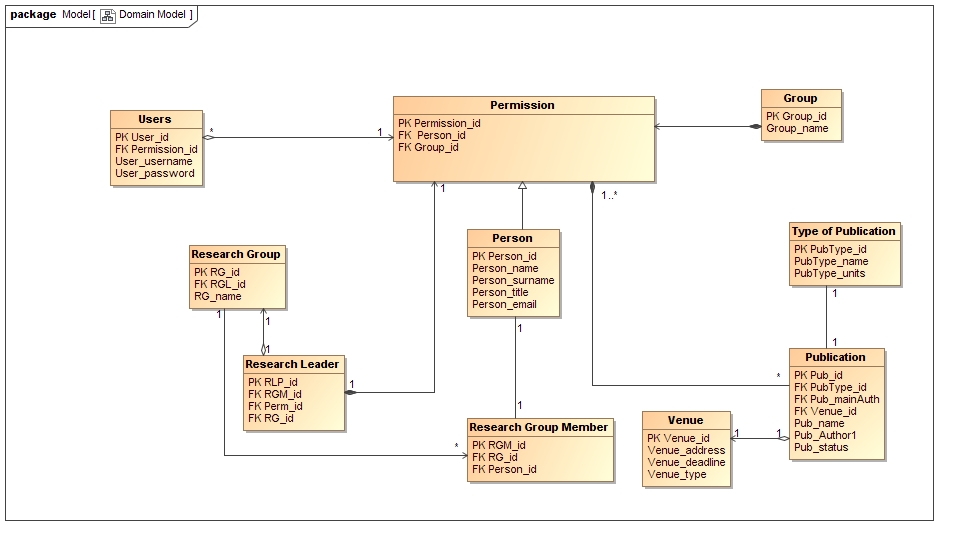
\includegraphics[width=\textwidth]{DomainModel.jpg}
		\caption{Domain Model of Research System \label{overflow}}
	\end{figure}
	\section{Open Issues}
	This section deals with issues that still need to be clarified, specified, assumed or have been discovered to include inconsistencies in the requirements, comprising of the following issues:
	\begin{description}
		\item[$\bullet$] Will a server be provided?
	\end{description}
	\begin{description}
		\item[$\bullet$] Should the HOD be a separate entity or fall within the Admin entity?
	\end{description}
	\begin{description}
	\item[$\bullet$] To where does the publication go to be reviewed?
	\end{description}
	\begin{description}
	\item[$\bullet$] Should the reminder system be via Mail or Calendar notification?
	\end{description}
	\begin{description}
	\item[$\bullet$] It is assumed that the Venue will have a deadline attached.
	\end{description}
		
\end{document}
